\documentclass[12pt,a4paper]{article}
\usepackage[utf8]{inputenc}
\usepackage{geometry}
\geometry{margin=1in}
\usepackage{enumitem}
\usepackage{titlesec}
\usepackage{graphicx}
\usepackage{float} 
\usepackage{hyperref} 
\usepackage{xcolor}
\usepackage{media9} 
\usepackage{hyperref}
\usepackage[table]{xcolor}

\title{Byte Me Application: Testing Evidence Report}
\author{Team Name: Byte Me}
\date{\today}

\begin{document}

\maketitle

\noindent \textbf{Testing Framework:} JUnit 5, Mockito, Spring Boot Test (DataJpaTest), MockMvc 

% --- Section 1: Security ---
\section{Security \& Authentication Testing (JwtUtilTest)}
\textbf{What was done:} 
\begin{itemize}
    \item Validated the generation and parsing of JSON Web Tokens (JWT).
    \item Tested the extraction of User ID, Email, and Role from encrypted payloads.
    \item Verified that expired tokens and malformed strings are correctly rejected.
\end{itemize}

\noindent \textbf{Justification:}
Security is our top priority. By testing the JWT system, we make sure that only the right users can log in and access their own data. This stops "identity spoofing," where someone might try to pretend to be another user to steal information or cause trouble.

\begin{figure}[H]
    \centering
    \includegraphics[width=0.7\linewidth]{Screenshot 2026-02-16 at 1.13.33 PM.png}
    \caption{JwtUtilTest: Validation of Secure Token Lifecycle}
\end{figure}

% --- Section 2: Inventory ---
\section{Inventory \& Transactional Logic (OrderControllerTest)}
\textbf{What was done:} 
\begin{itemize}
    \item Simulated successful order creation and stock reservation.
    \item Tested edge cases, specifically prevent orders when stock is insufficient.
    \item Verified the full lifecycle of an order: \texttt{RESERVED} $\rightarrow$ \texttt{COLLECTED} or \texttt{RESERVED} $\rightarrow$ \texttt{CANCELLED}.
\end{itemize}

\noindent \textbf{Justification:}
When dealing with food rescue, accurate numbers are vital. We don't want a charity to show up for food that isn't there. This testing fixes the "double-booking" problem at the source and ensures that if someone cancels an order, the food automatically goes back on the list for someone else to claim.

\begin{figure}[H]
    \centering
    \includegraphics[width=0.7\linewidth]{OrderControllerTest.png}
    \caption{OrderController: Transactional Stock Management Evidence}
\end{figure}

\begin{figure}[H]
    \centering
    \includegraphics[width=0.7\linewidth]{FullFlowIntegrationTest.png}
    \caption{Full Flow Integration: Validating the path from Reservation to Collection}
\end{figure}

% --- Section 3: CI/CD ---
\section{Automated CI/CD Pipeline Integration}
\textbf{What was done:} 
\begin{itemize}
    \item Configured Railway's native CI/CD integration with the GitHub repository.
    \item Established an automated trigger that initiates the deployment pipeline upon every commit.
    \item Integrated the execution of the full JUnit test suite as a mandatory build step.
\end{itemize}

\noindent \textbf{Justification:}
We use Railway and GitHub to check our code quality automatically every time we save our work. This "feedback loop" means the computer double-checks our tests for us. It helps catch human mistakes early and guarantees that the live app is always using a stable, working version.

\begin{figure}[H]
    \centering
    \includegraphics[width=0.9\linewidth]{GitHubActionPage.png}
    \caption{Railway CI/CD Pipeline: Automated Test Suite Execution Logs}
\end{figure}

% --- Section 4: Data Integrity ---
\section{Data Integrity \& Persistence (Repository Tests)}
\textbf{What was done:} 
\begin{itemize}
    \item Used \texttt{@DataJpaTest} to verify the schema constraints (Unique emails, Not Null names).
    \item Verified custom query methods, such as finding issues by Seller ID.
    \item Tested the immutability of \texttt{createdAt} timestamps using \texttt{updatable = false} validation.
\end{itemize}

\noindent \textbf{Justification:}
The database is where all our important information lives. These tests make sure the "rules" of our data are followed—like making sure two people don't sign up with the same email. This prevents "dirty data" from getting into the system, which would otherwise cause the app to crash later on.

\begin{figure}[H]
    \centering
    \includegraphics[width=0.7\linewidth]{Screenshot 2026-02-16 at 10.38.29 PM.png}
    \caption{Repository Layer: Database Constraint and Query Validation}
\end{figure}

% --- Section 5: Gamification ---
\section{Gamification \& Engagement (GamificationControllerTest)}
\textbf{What was done:} 
\begin{itemize}
    \item Mocked the retrieval of user streaks (Current and Best).
    \item Verified the logic for awarding badges like \texttt{STREAK\_4} and \texttt{CO2\_SAVER}.
    \item Tested DTO mapping to ensure the frontend receives correctly formatted JSON.
\end{itemize}

\noindent \textbf{Justification:}
We use a streak system to encourage users to keep donating and rescuing food. Testing this ensures the game is "fair"—streaks should only go up when a user actually completes a task. This keeps users engaged and ensures they get the badges they've actually earned.

\begin{figure}[H]
    \centering
    \includegraphics[width=0.48\linewidth]{OrganisationBadgeTest.png}
    \includegraphics[width=0.48\linewidth]{OrganisationStreakCacheTest.png}
    \caption{Gamification: Badge Award Logic and Streak Persistence}
\end{figure}

% --- Section 6: Issues ---
\section{Issue Reporting \& Conflict Resolution (IssueControllerTest)}
\textbf{What was done:} 
\begin{itemize}
    \item Verified that Organisations can report issues with orders.
    \item Tested the ``Resolve'' flow and automatic generation of resolution timestamps.
\end{itemize}

\noindent \textbf{Justification:}
Trust is the key to a successful marketplace. If there is a problem with an order, we need a reliable way to track and fix it. These tests ensure that every complaint is recorded and that there is a clear "paper trail" showing when and how a problem was solved.

\begin{figure}[H]
    \centering
    \includegraphics[width=0.7\linewidth]{Screenshot 2026-02-16 at 10.33.46 PM.png}
    \caption{IssueController: Audit Trail and Dispute Resolution Testing}
\end{figure}

% --- Section 7: Entities ---
\section{Domain Model Validation (Entity Tests)}
\textbf{What was done:}
\begin{itemize}
    \item Tested Pojos like \texttt{UserAccount}, \texttt{Seller}, and \texttt{Organisation}.
    \item Verified that default values are assigned upon object instantiation.
\end{itemize}

\noindent \textbf{Justification:}
Entities are the basic building blocks of our app. We test them to make sure the "foundation" is solid. If the simple things don't work, the complex parts of the app won't work either. This keeps our data consistent from the start.

\begin{figure}[H]
    \centering
    \includegraphics[width=0.45\linewidth]{UserAccountTest.png}
    \includegraphics[width=0.45\linewidth]{SellerTest.png}
\end{figure}
\begin{figure}[H]
    \centering
    \includegraphics[width=0.45\linewidth]{OrganisationTest.png}
    \includegraphics[width=0.45\linewidth]{ReservationTest.png}
    \caption{Entity Validation: Ensuring structural integrity of core Domain Objects}
\end{figure}


% --- Section 8: Frontend UI & Component Testing ---
\section{Frontend UI \& Component Testing (Vitest / React Testing Library)}
\textbf{What was done:} 
\begin{itemize}
    \item \textbf{Feature-Specific Validation:} Executed 191 automated tests across 13 core modules, including \texttt{Seller Dashboard}, \texttt{Organization Gamification}, and \texttt{Bundle Management}.
    \item \textbf{User Flow Simulation:} Verified complex user interactions such as \texttt{create-bundle} workflows and \texttt{seller-analytics} data visualization.
    \item \textbf{Authentication \& Registration:} Tested the integrity of the \texttt{login} and \texttt{register} components, ensuring proper validation and secure redirection.
    \item \textbf{Role-Based Logic:} Validated unique views for both \texttt{Seller} and \texttt{Organization} roles, ensuring data isolation and relevant dashboard metrics.
\end{itemize}

\noindent \textbf{Justification:}
The frontend is the primary touchpoint for our users. By running a comprehensive suite of 191 tests, we ensure that the UI behaves predictably across different devices and user roles. This prevents "regression bugs" and guarantees that the environmental impact data and gamification badges are displayed accurately.

\begin{figure}[H]
    \centering
    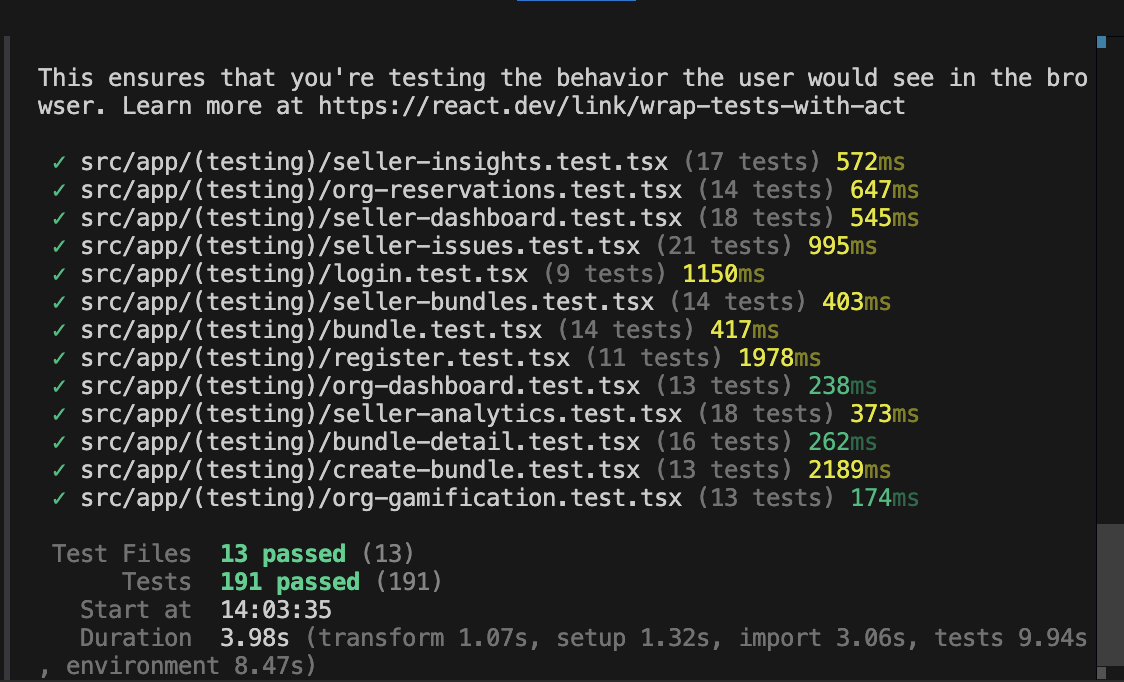
\includegraphics[width=0.9\linewidth]{Frontend Test screenshot.png}
    \caption{Frontend Test Execution: 191 Passed Tests across 13 Suites}
\end{figure}


% --- Section 9: Manual Testing & Video Evidence ---
\newpage
\section{Manual End-to-End Testing}

\textbf{Requirement:} This section provides explicit evidence of manual testing, including failure cases and edge cases.

% Case 1
\subsection{TC-01: Failure Case - Invalid Authentication}
\textbf{Scenario:} User attempts to log in with a valid email but an incorrect password. \\
\textbf{Expected Result:} The system identifies the mismatch and displays an "Invalid credentials" error message. \\
\begin{figure}[H]
    \centering
    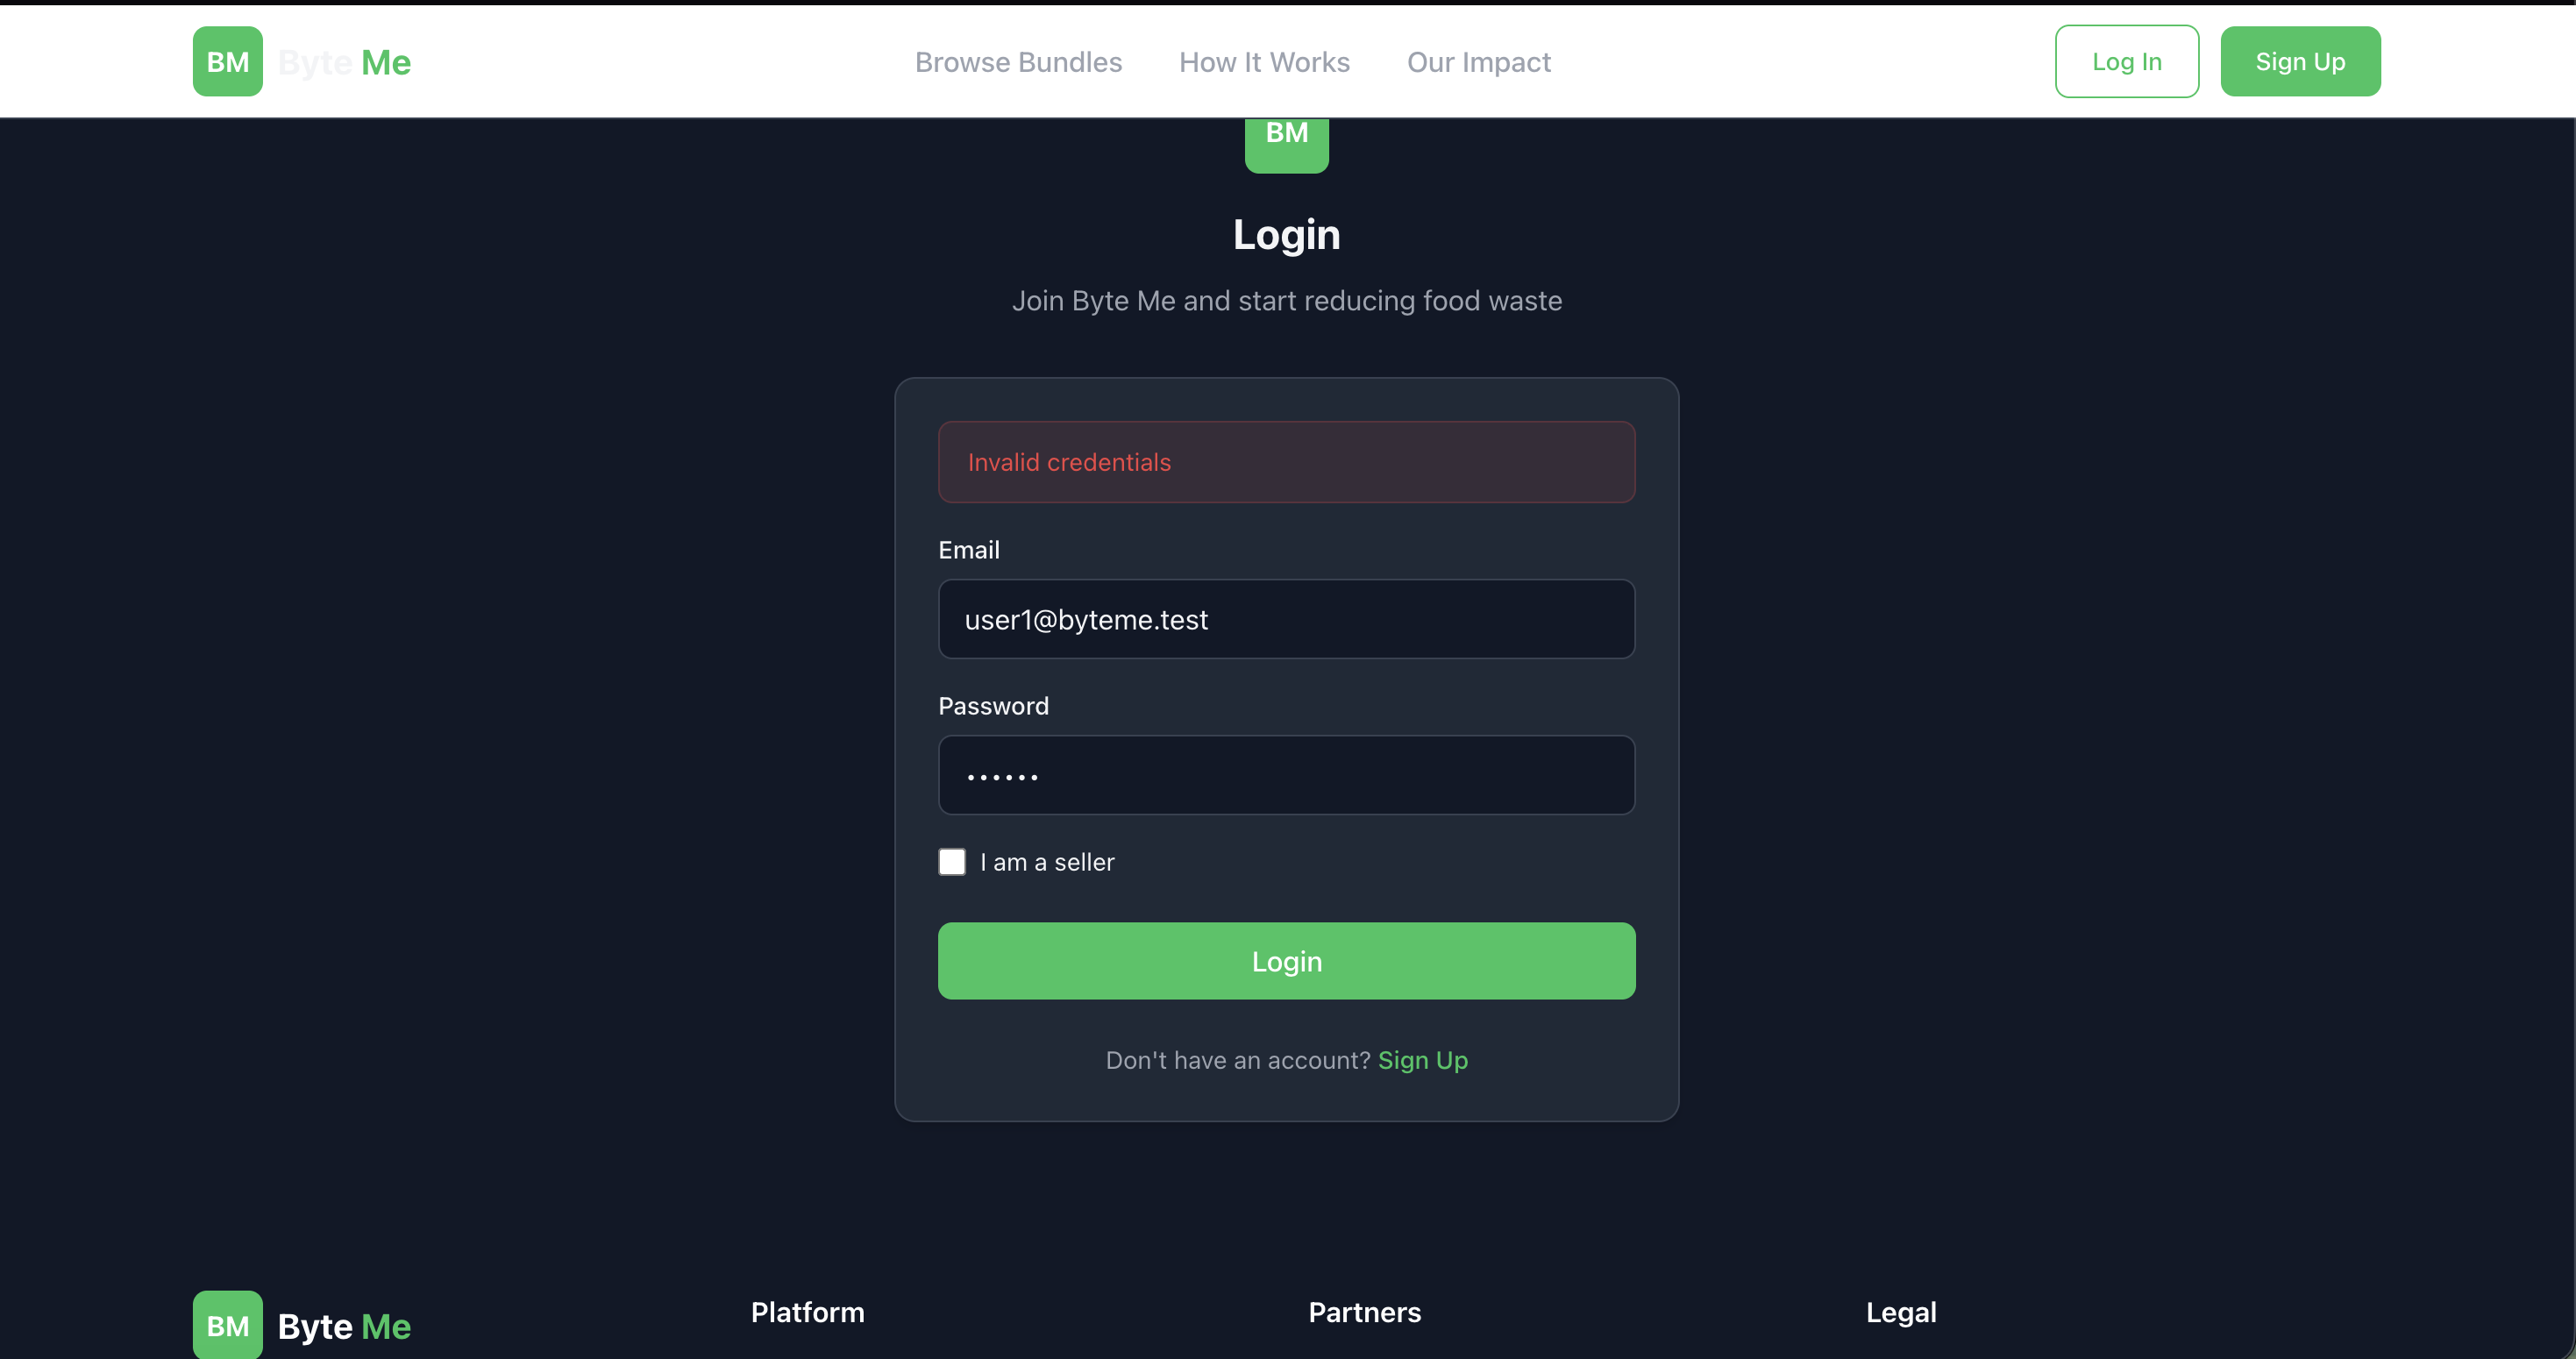
\includegraphics[width=0.85\linewidth]{invaild login.png}
    \caption{UI Evidence: Authentication failure feedback.}
\end{figure}

% Case 2

\subsection{TC-02: Failure Case - Negative Value Input Validation}
\textbf{Scenario:} Seller attempts to set a negative price (-10) during bundle creation. \\
\textbf{Expected Result:} The UI prevents the form submission and displays a validation tooltip. \\
\begin{figure}[H]
    \centering
    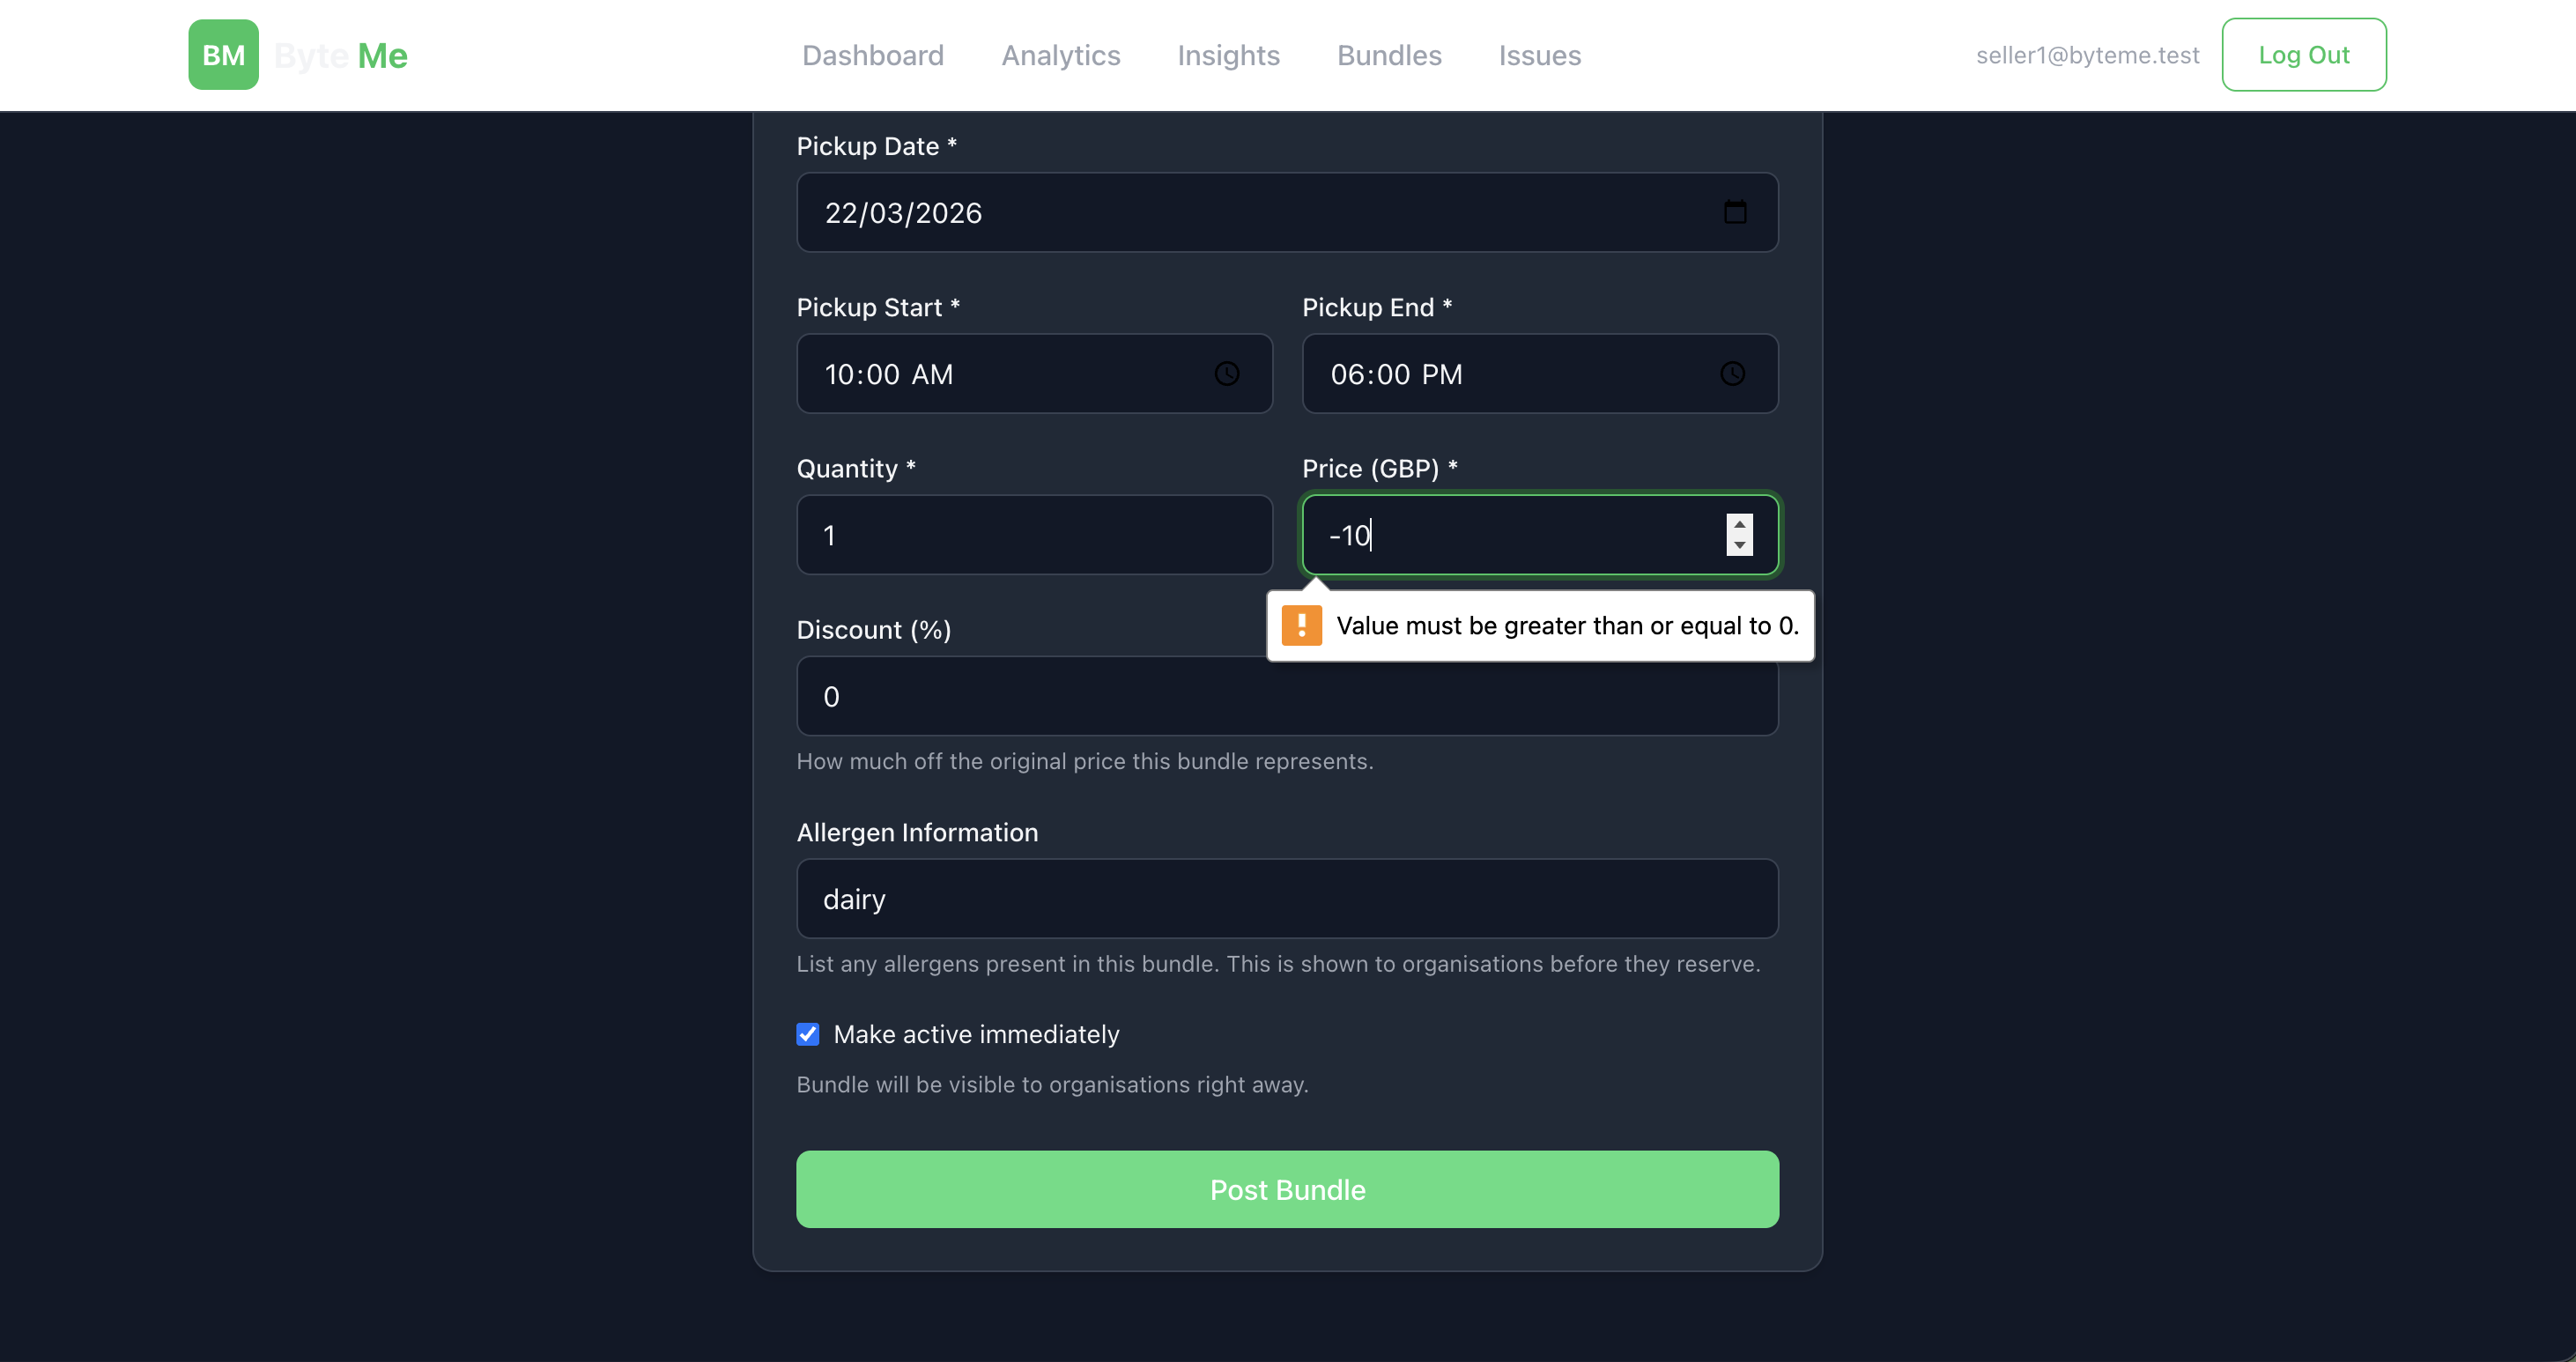
\includegraphics[width=0.85\linewidth]{Can not eneter invaild numbers.png}
    \caption{UI Evidence: Frontend validation for numeric constraints.}
\end{figure}

% Case 3 
\subsection{TC-03: Failure Case - Race Condition (Concurrent Reservation)}
\textbf{Scenario:} Two users attempt to reserve the final available bundle simultaneously. User A's request processes milliseconds earlier. \\
\textbf{Expected Result:} The system must maintain strict inventory integrity. While the first user succeeds, the second user (User B) must receive a "No bundles available" error, preventing a negative stock balance. \\
\begin{figure}[H]
    \centering
    \includegraphics[width=0.85\linewidth]{No bundle avaliable after one person reserve it first.png}
    \caption{UI Evidence: Real-time inventory check preventing overselling after a concurrent claim.}
\end{figure}

% Case 5
\subsection{TC-05: Edge Case - Reservation Cancellation}
\textbf{Scenario:} User clicks the 'Cancel' button on an active reservation. \\
\textbf{Expected Result:} A browser modal confirms the action to prevent accidental data loss. \\
\begin{figure}[H]
    \centering
    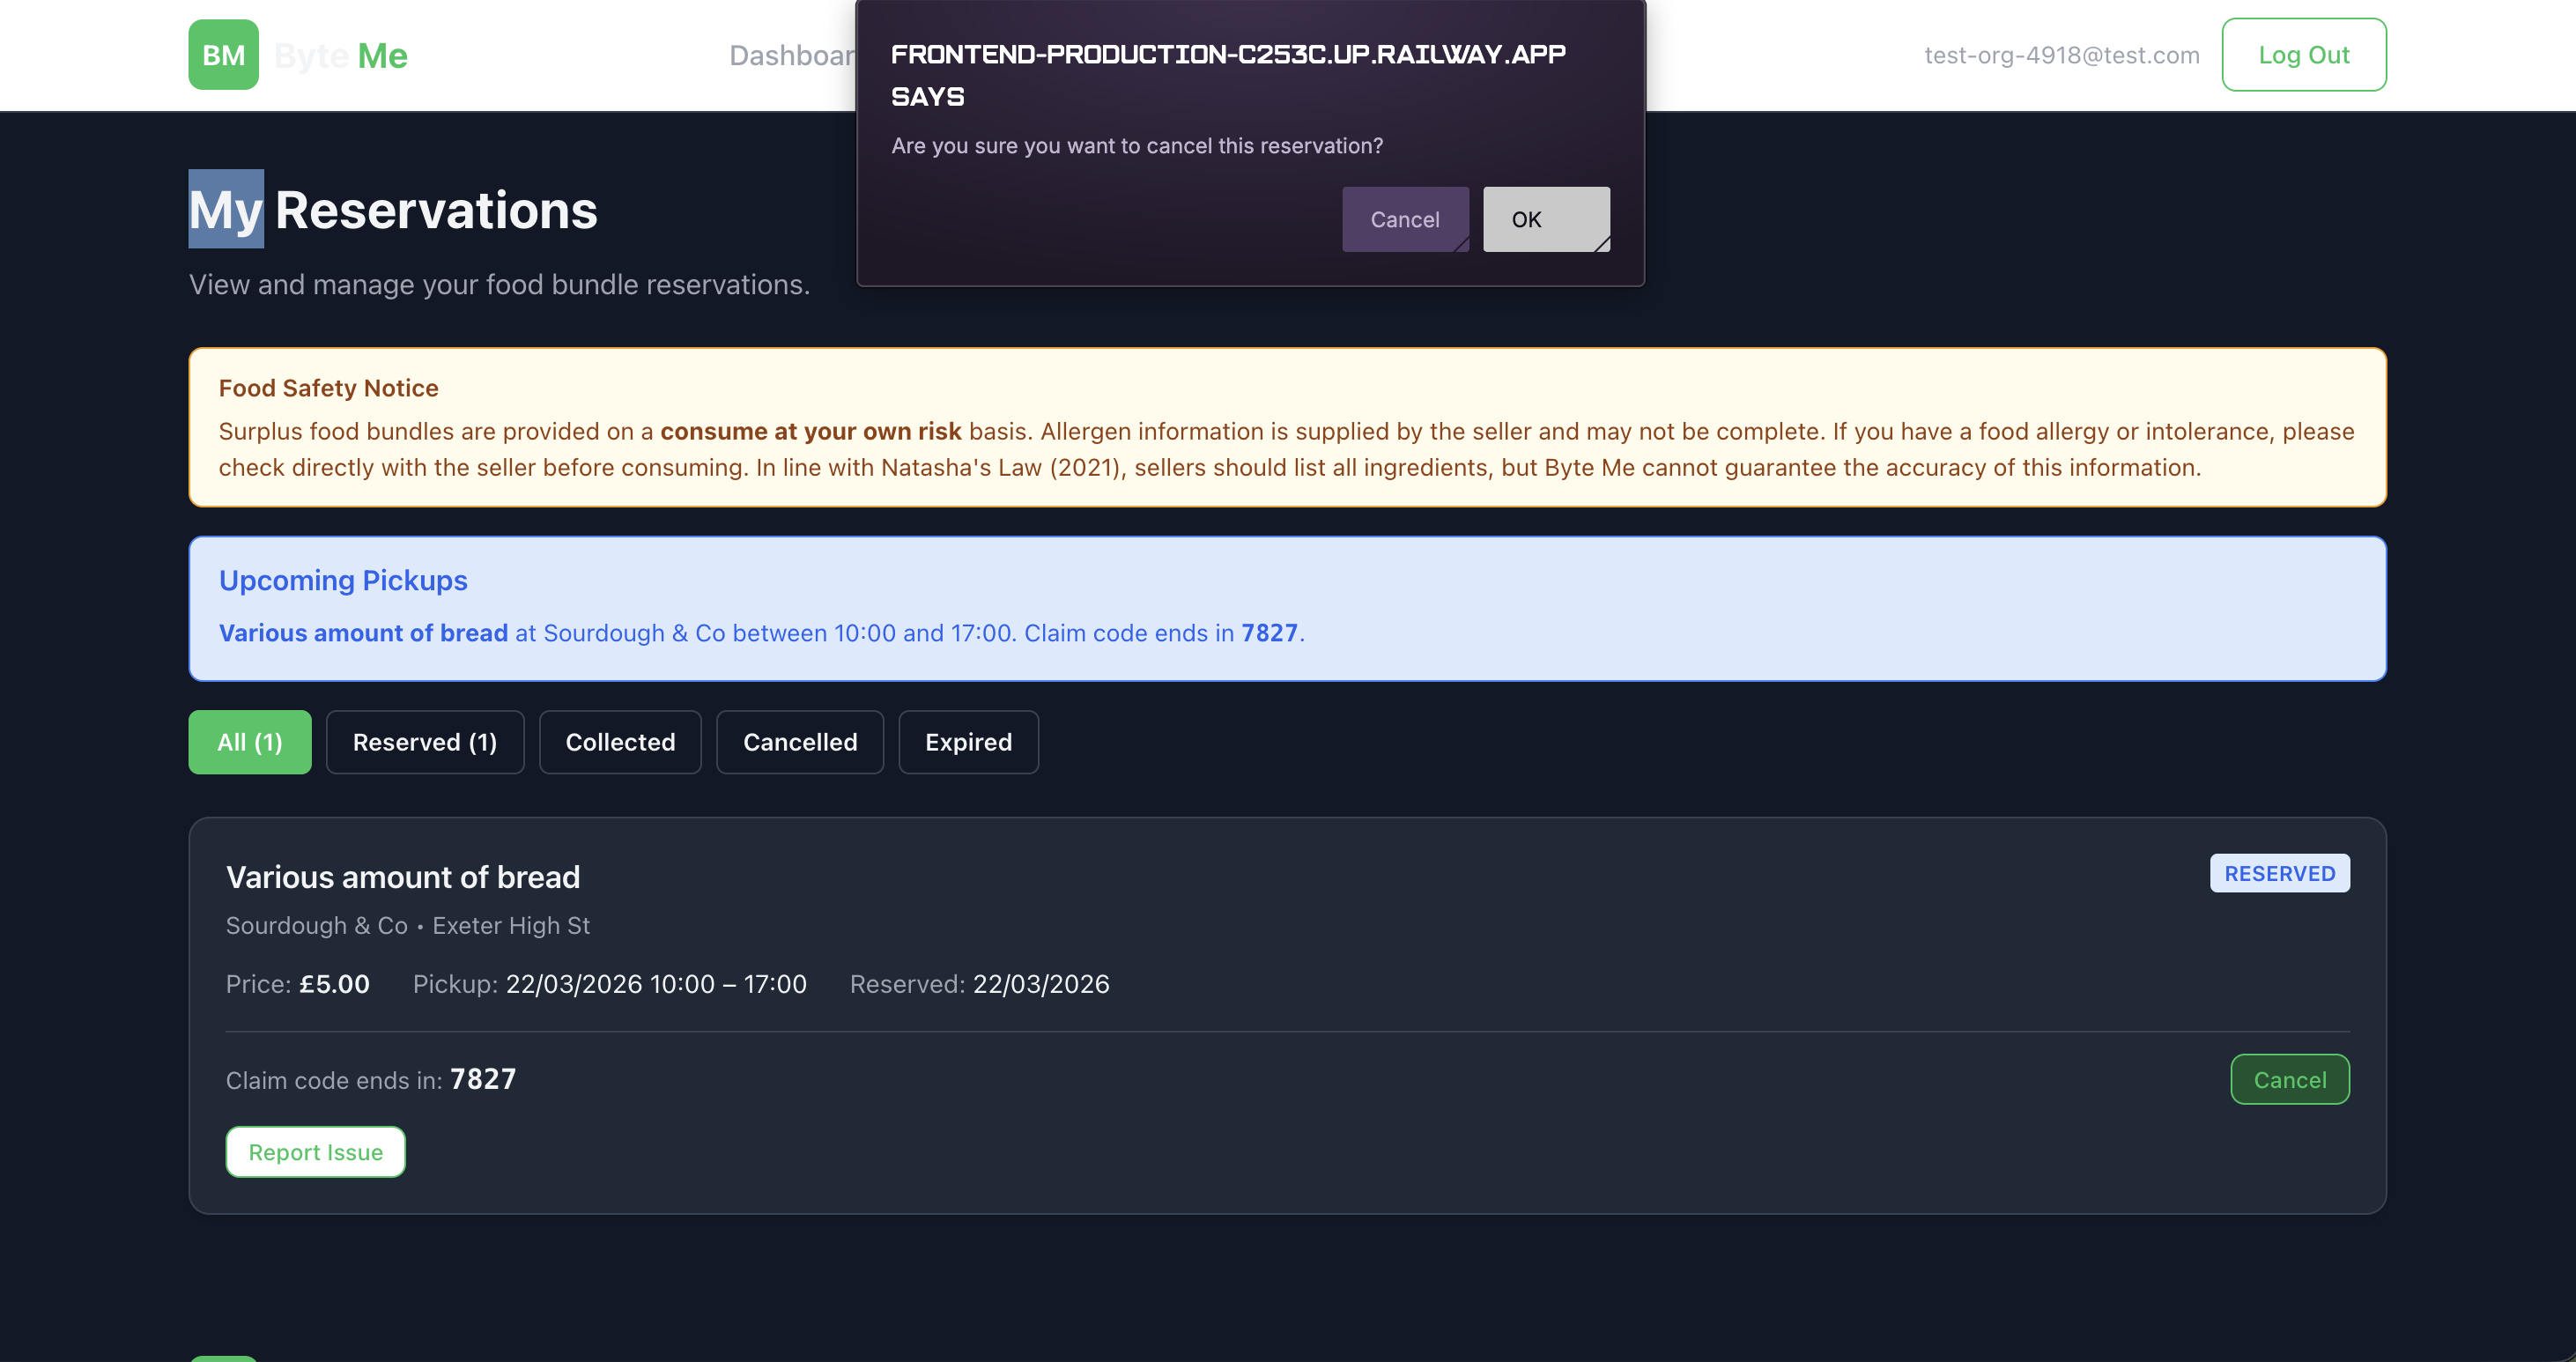
\includegraphics[width=0.85\linewidth]{cancel the reserve.png}
    \caption{UI Evidence: Safety modal for state-changing actions.}
\end{figure}

% Case 6
\subsection{TC-06: State Integrity - Sold Out Logic}
\textbf{Scenario:} A bundle reaches 0 availability. \\
\textbf{Expected Result:} The bundle details page replaces the action button with a "Sold Out" status. \\
\begin{figure}[H]
    \centering
    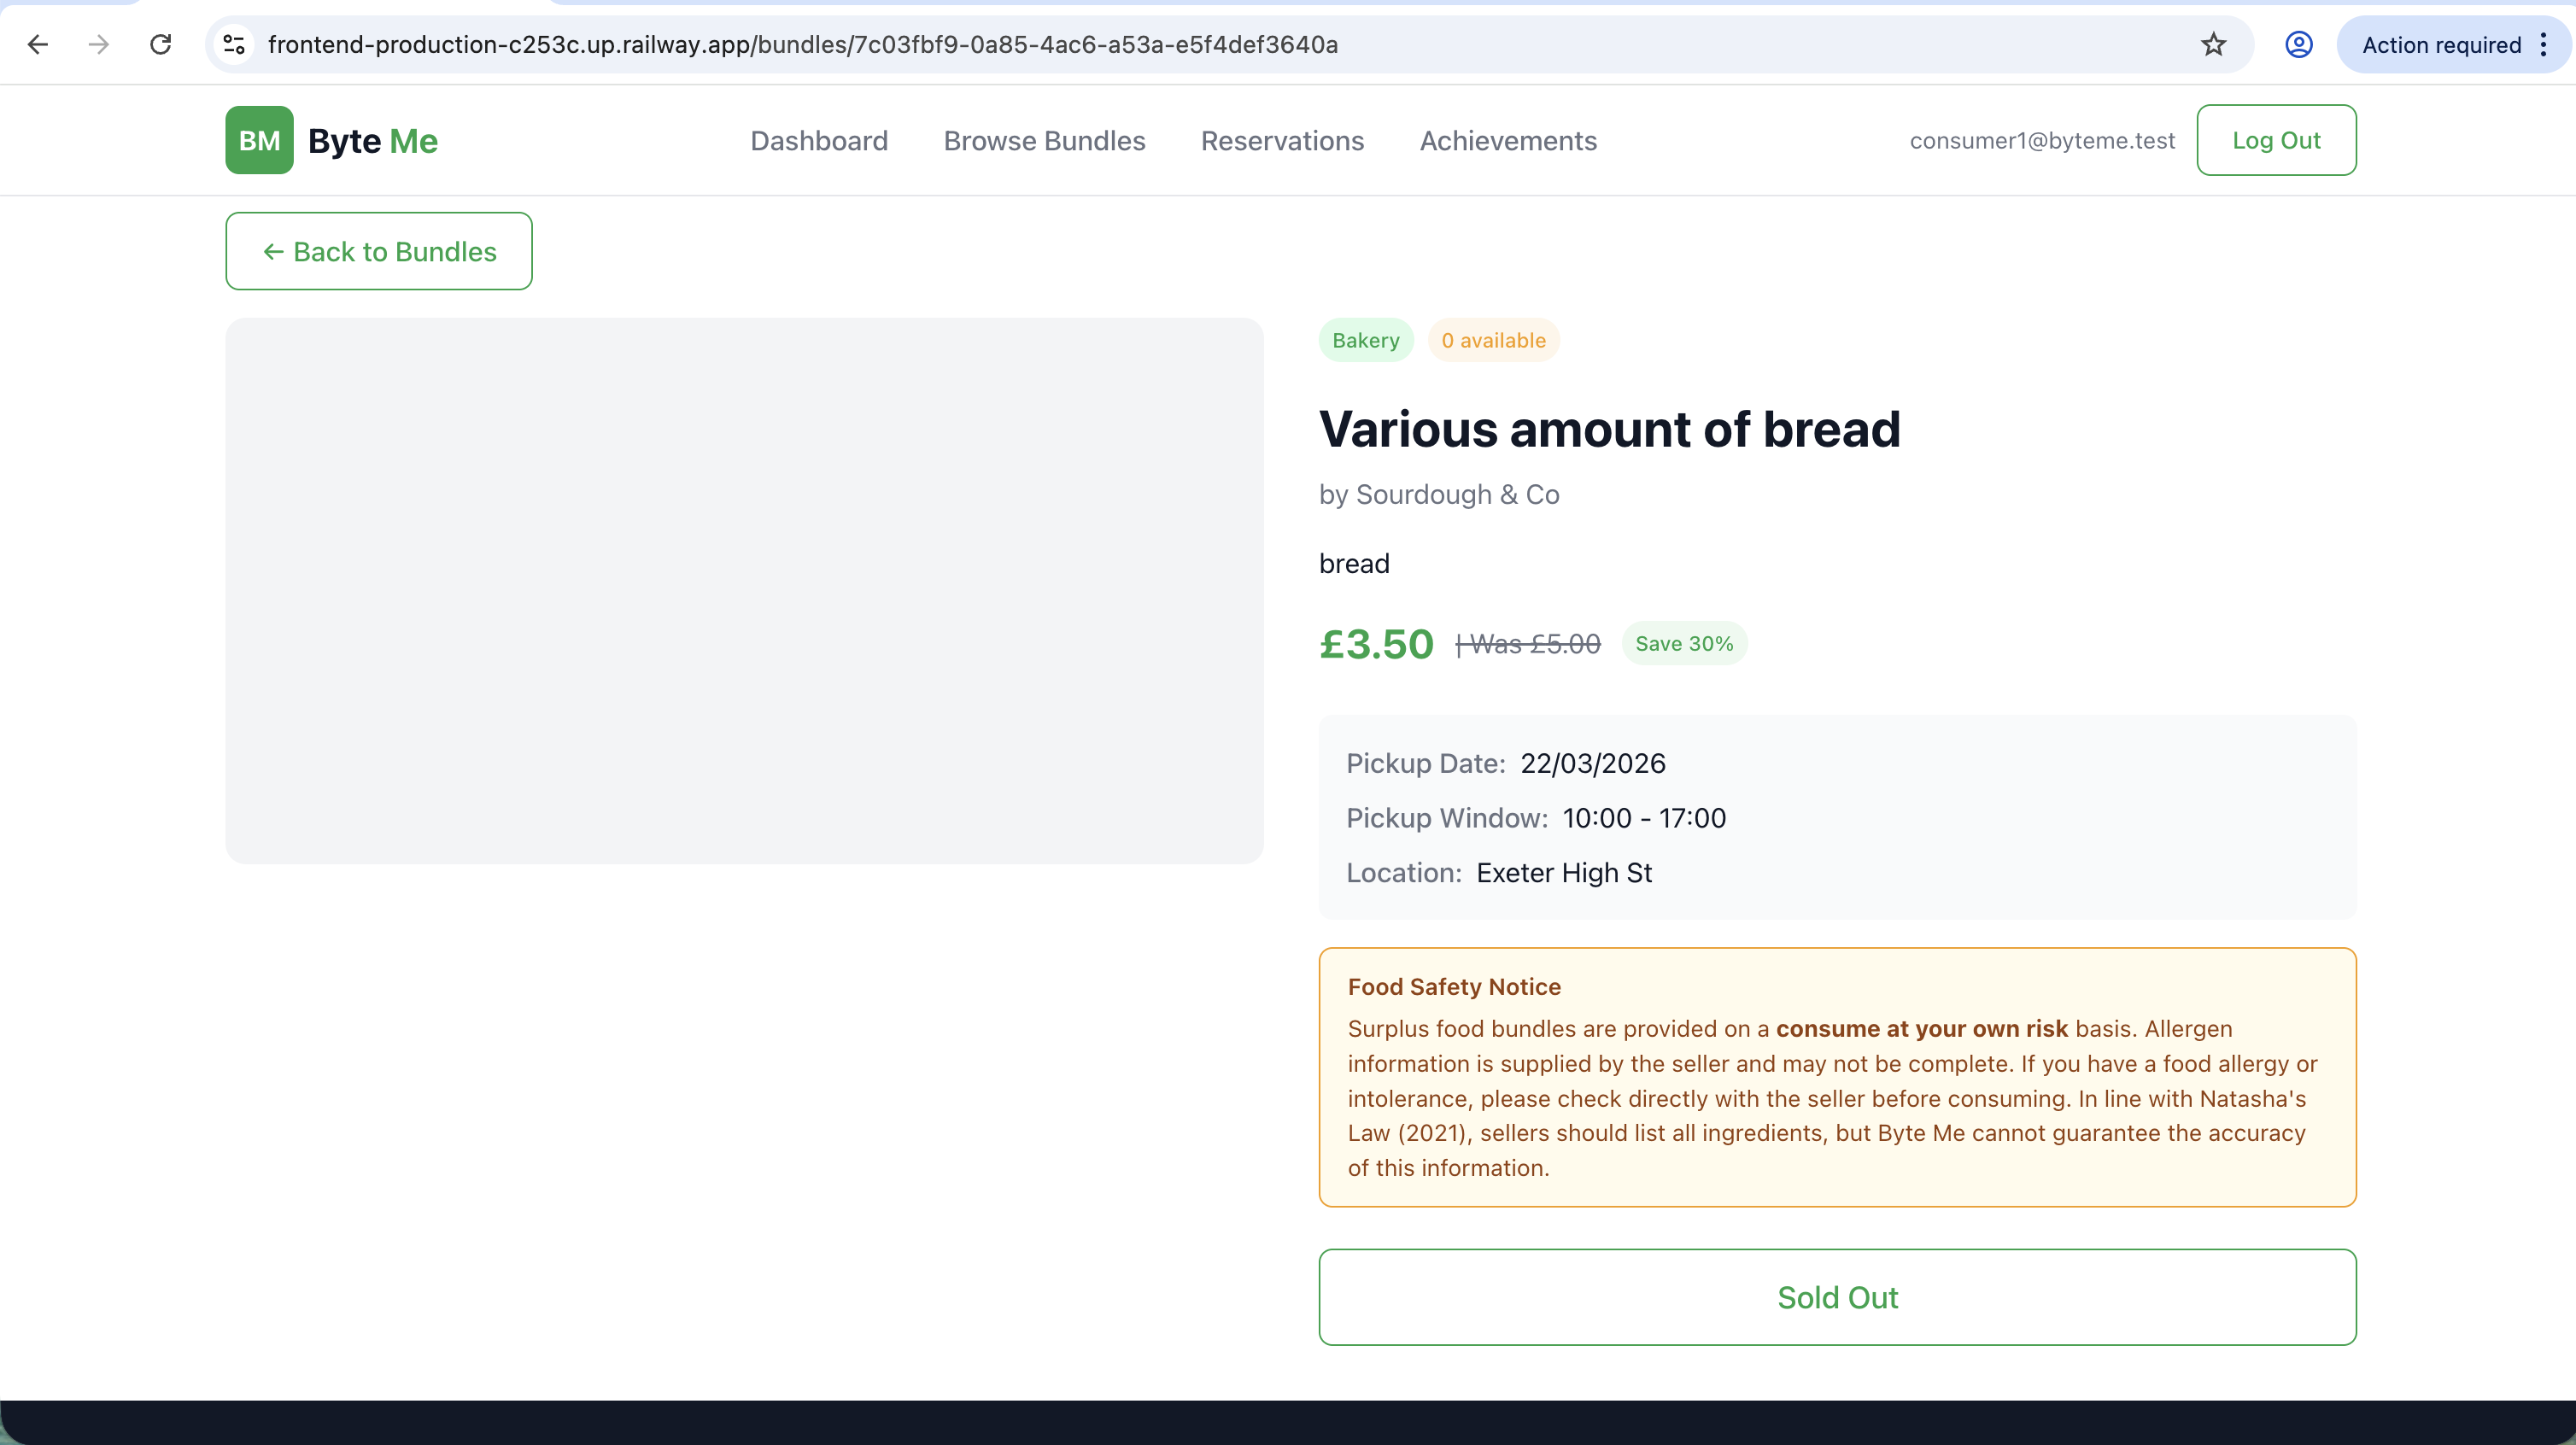
\includegraphics[width=0.85\linewidth]{Sold Out Bundle.png}
    \caption{UI Evidence: Automated status update based on inventory.}
\end{figure}


\subsection{Manual User Acceptance Testing (Happy Case Video Evidence)}
\textbf{Overview:} 
To complement our automated suite, we performed an end-to-end manual walkthrough of the system's \textbf{Happy Path} (the ideal user journey where no errors occur). This recording demonstrates the successful live synchronization between the Seller and Organization (Consumer) roles, confirming the full cycle of a food bundle from creation to collection.

\noindent \textbf{Justification:}
This video acts as a comprehensive "walkthrough" of the successful transaction flow. By recording these happy path scenarios, we prove that the integration between the frontend UI and the Spring Boot backend is seamless and that the database correctly handles valid transactional changes in a live environment.

\subsection*{Happy Path: Walkthrough Key Actions \& Timestamps}
\begin{table}[H]
    \centering
    \small
    \renewcommand{\arraystretch}{1.2}
    \begin{tabular}{|l|p{8cm}|c|}
        \hline
        \rowcolor{gray!10} \textbf{Phase (Happy Path)} & \textbf{Successful Action Performed} & \textbf{Timestamp} \\ \hline
        \textbf{Registration} & Seller Sign-up: Creating a business profile & [00:05] \\ \cline{2-3}
        & Organization Sign-up: Creating a consumer profile & [00:30] \\ \hline
        \textbf{Seller Flow} & Profile Navigation: Viewing settings and dashboard & [00:36] \\ \cline{2-3}
        & \textbf{Bundle Creation:} Successfully posting food surplus & [01:00] \\ \hline
        \textbf{Organization} & Listing Discovery: Browsing available bundles & [02:40] \\ \cline{2-3}
        \textbf{Workflow} & \textbf{Reservation:} Booking a bundle and generating code & [02:50] \\ \cline{2-3}
        & Active Claims: Viewing reservations tab & [03:00] \\ \cline{2-3}
        & \textbf{Order Integrity:} Re-booking and new code generation & [04:00] \\ \hline
        \textbf{Collection} & \textbf{Handover:} Using confirmation code for pickup & [04:06] \\ \cline{2-3}
        & Seller Dashboard: Verifying "Collected" status & [04:20] \\ \cline{2-3}
        & Consumer Dashboard: Final status update verification & [04:30] \\ \hline
        \textbf{Persistence} & \textbf{Session Management:} Logging out and back in successfully & [05:00] \\ \hline
        \textbf{Impact} & \textbf{Success Metrics:} Viewing CO2 and forecast stats & [05:18] \\ \cline{2-3}
        & \textbf{Achievements:} Reviewing "First Rescue" badge & [05:35] \\ \hline
    \end{tabular}
    \caption{Manual Testing Time-Log: Successful (Happy Path) Integration}
\end{table}

\begin{figure}[H]
    \centering
    \includemedia[
      width=0.9\linewidth,
      height=0.5\linewidth,
      activate=onclick,
      addresource=Manual Testing.mp4, 
      flashvars={source=Manual Testing.mp4 & autoPlay=false}
    ]{ \includegraphics[width=0.9\linewidth]{video_poster.png} }{VPlayer.swf}
    \caption{Happy Path Demonstration: Live Application Walkthrough}
\end{figure}

\noindent \textbf{Note:} To play the embedded video, please open this PDF in \textbf{Adobe Acrobat Reader}. Alternatively, access the video via the direct link below:

\begin{center}
    \url{https://youtu.be/5NwwiJ71_DY}
\end{center}

\end{document}